\documentclass[10pt,letterpaper]{article}
\usepackage[lmargin=2.2in,rmargin=0.7in,tmargin=1.0in,bmargin=1.0in]{geometry}
\usepackage{notes}
\begin{document}


\begin{center}
\Large\textbf{2.5 - Unforced Springs}\\
\normalsize (Section 2.2.4)
\end{center}


%-------------------------------------------------------------
\section{Spring Classification}

In this section, we explain all the possible solutions that can be obtained from the spring-mass equation. The fact that the coefficients are all non-negative imposes a restriction on the types of solutions.

\subsection{Eigenvalues for Springs}
The spring--mass equation describes the displacement $x(t)$
of a ball from equilibrium:
\[
mx''+\gamma x'+kx=0,
\]
where $m>0$ is the \textbf{mass}, $k>0$ is the
\textbf{spring constant}, and $\gamma\ge0$ is the
\textbf{damping coefficient}. These restrictions limit the
possible behavior of the solutions. The characteristic equation and its roots are
\[
m\lambda^2+\gamma\lambda+k=0,
\qquad
\lambda_{1,2}
=\frac{-\gamma\pm\sqrt{\gamma^2-4mk}}{2m}.
\]
We will consider three cases based on the sign of the
discriminant $D=\gamma^2-4mk$.



\subsection{Case: Positive Discriminant}
If $D>0$, there are two real, distinct eigenvalues:
\[
\lambda_1=\frac{-\gamma+\sqrt{\gamma^2-4mk}}{2m},
\qquad
\lambda_2=\frac{-\gamma-\sqrt{\gamma^2-4mk}}{2m}.
\]
In this case, $\gamma>0$, so $\lambda_2<0$.
The sign of $\lambda_1$ is less obvious because its numerator
contains both a negative and a positive term. However, we can prove that $\lambda_1$ is always negative.

\begin{proof}
Suppose, for a contradiction, that $\lambda_1\ge0$. Then
\begin{align*}
\frac{-\gamma+\sqrt{\gamma^2-4mk}}{2m}&\ge0\\
\sqrt{\gamma^2-4mk}&\ge\gamma\\
\gamma^2-4mk&\ge\gamma^2\\
-4mk&\ge0.
\end{align*}
This contradicts $m>0$ and $k>0$. Therefore, $\lambda_1<0$.
\end{proof}
If $D>0$, the solution to the spring-mass equation must be a sum of exponential decays
\[
x(t)=
\underbrace{c_1e^{\lambda_1t}}_{\text{decay}}
+\underbrace{c_2e^{\lambda_2t}}_{\text{decay}}.
\]
Physically, the ball approaches equilibrium without repeated
oscillations. We call this an \textbf{overdamped} system.
The damping is strong enough to prevent repeated swinging.

\subsection{Case: Zero Discriminant}

If $D=0$, there is a repeated eigenvalue
\[
\lambda=-\frac{\gamma}{2m}<0.
\]
The solution is a linear factor multiplied by an exponential decay:
\[
x(t)=(c_1+c_2t)\underbrace{e^{\lambda t}}_{\text{decay}}.
\]
The ball approaches equilibrium without repeated oscillations.
We call this a \textbf{critically damped} system. Depending on the initial conditions, it may cross equilibrium once or not at all. 

\subsection{Case: Negative Discriminant}

If $D<0$, the eigenvalues are complex:
\[
\lambda_{1,2}
=
\underbrace{-\frac{\gamma}{2m}}_{\alpha}
\pm i\underbrace{\frac{\sqrt{4mk-\gamma^2}}{2m}}_{\beta}.
\]
The real part $\alpha$ is negative or zero. If $\gamma>0$, then $\alpha<0$, and the solution is a wave multiplied by an exponential decay:
\[
x(t)=
\underbrace{e^{\alpha t}}_{\text{decay}}
\underbrace{(c_1\cos\beta t+c_2\sin\beta t)}_{\text{wave}}.
\]
The ball bounces back and forth with decreasing amplitude.
The damping weakens the motion but is not strong enough
to prevent oscillation. We call this an
\textbf{underdamped} system. In the ideal model, the swings
continue indefinitely while becoming smaller and smaller.

If $\gamma=0$, there is no damping. The eigenvalues are
purely imaginary:
\[
\lambda_{1,2}=\pm i\sqrt{\frac{k}{m}}.
\]
The exponential factor is now $e^{0t}=1$, so the solution is
\[
x(t)=c_1\cos\beta t+c_2\sin\beta t,
\qquad \beta=\sqrt{\frac{k}{m}}.
\]
The ball bounces back and forth with constant amplitude.
We call this an \textbf{undamped} system because no damping
force removes energy from the motion.

\subsection{Summary of Classifications}
You are responsible for knowing the \textbf{four types of
spring motion}: overdamped, critically damped, underdamped,
and undamped. Mathematically, we classify the system using the discriminant
$D=\gamma^2-4mk$ and whether $\gamma=0$.
Physically, these classifications describe how much damping
is present relative to the critical level and whether the
ball repeatedly bounces back and forth. The four classifications are summarized in the table below. 

\begin{center}
\renewcommand{\arraystretch}{1.6}
\setlength{\tabcolsep}{6pt}

\begin{tabularx}{\textwidth}{|>{\centering\arraybackslash}X|>{\centering\arraybackslash}X|c|c|>{\centering\arraybackslash}X|>{\centering\arraybackslash}X|}
\hline
\textbf{Classification} & \textbf{Condition} & \textbf{Example} & \textbf{Sketch} &\textbf{Friction} & \textbf{Behavior}\\
\hline
Over- damped 
& $D>0$
& $x = e^{-t}$ 
& \tikz[baseline=-0.5ex,scale=0.45]{
    \draw[->] (0,0) -- (2,0);
    \draw[->] (0,-1) -- (0,1.1);
    \draw[thick,domain=0:2,samples=60]
        plot (\x,{1.0*exp(-1.4*\x)});
} &Too much & No swinging
\\
\hline

Critically Damped 
& $D=0$
& $x = (-2t+1)e^{-t}$
& \tikz[baseline=-0.5ex,scale=0.45]{
    \draw[->] (0,0) -- (2,0);
    \draw[->] (0,-1.1) -- (0,1.1);
    \draw[thick,domain=0:2,samples=80]
        plot (\x,{(0.5-4*\x)*exp(-2*\x)});
}& Tipping point
&
One swing
\\
\hline

Under- damped 
& $D<0,$ $\gamma\neq0$
& $x = e^{-t}\cos t$
& \tikz[baseline=-0.5ex,scale=0.45]{
    \draw[->] (0,0) -- (2,0);
    \draw[->] (0,-1.1) -- (0,1.1);
    \draw[thick,domain=0:2,samples=120]
        plot (\x,{exp(-0.5*\x)*cos(deg(6*\x))});
    \draw[dashed,domain=0:2]
        plot (\x,{exp(-0.5*\x)});
    \draw[dashed,domain=0:2]
        plot (\x,{-exp(-0.5*\x)});
}& Too little
&
Few swings
\\
\hline
Undamped 
& $\gamma=0$
& $x = \cos t$
& \tikz[baseline=-0.5ex,scale=0.45]{
    \draw[->] (0,0) -- (2,0);
    \draw[->] (0,-1.1) -- (0,1.1);
    \draw[thick,domain=0:2,samples=120]
        plot (\x,{cos(deg(6*\x))});
} & none
&
Infinite swinging
\\
\hline

\end{tabularx}
\end{center}

\begin{example}[1]{
A mass of $m=5$ kg is attached to a spring with stiffness
$k=2$ N/m and damping coefficient $\gamma=5$ kg/s.
Classify the spring-mass system.
}
The spring-mass equation is
\[
5x''+5x'+2x=0.
\]
Its characteristic equation is
\[
5\lambda^2+5\lambda+2=0,
\]
with discriminant
\[
D=\gamma^2-4mk=5^2-4(5)(2)=-15<0.
\]
Since $D<0$ and $\gamma>0$, the system is
\[
\boxed{\text{underdamped}.}
\]
\end{example}


%-------------------------------------------------------------
\section{Parameter Dependent Models}

\subsection{Parameters}
\textbf{Parameters} are quantities held fixed during a particular
experiment, but which may differ between experiments. Pretend you are an experimentalist conducting tests on the spring-mass system. In the model
\[
\begin{dcases}
m x'' + \gamma  x' + kx = 0,\\
x(0)=x_0\\
x'(0)=v_0,
\end{dcases}
\]
you control 5 parameters:  mass $m$, the stiffness $k$, the initial pull $x_0$, the initial velocity $v_0$, and possibly the friction $\gamma$. The solution $x(t)$ is not a parameter. We call $x(t)$ the \textbf{response} because it is the resulting behavior that results from our choice of parameters.

Changing $x_0$ or $v_0$ changes the particular motion, but it
does not change the \textit{damping classification}. For example,
a critically damped system remains critically damped regardless
of the initial displacement or velocity. The damping classification depends purely on $m$, $\gamma$, and $k$.

\begin{example}[2]{    
Suppose you have a spring with stiffness $k=2$ kg/$s^2$. You are able to freely control the mass of the ball, but the damping coefficient scales with the mass: $\gamma=2m$. What would the mass of the ball need to be for underdamped oscillations? 
}

Start by writing the model:
\begin{align*}
    m\,x'' + 2m\, x' + 2x &= 0.
\end{align*}
Next, we find the discriminant 
$$
D = b^2-4ac = 4m^2 -8m = 4m(m-2).
$$
For underdamped, we set $D<0$. Since $m>0$, we can divide by $4m$ without reversing
the inequality:
\[
4m(m-2)<0
\quad\Rightarrow\quad
m-2<0.
\]
Therefore, the system is underdamped when
\[
\boxed{0<m<2.}
\]
\end{example}

\subsection{Parameter Space}

In Example 2, the mass $m$ entirely controls the oscillation type of the spring. Thus, we can represent the possible systems as points on a number line, which we call the \textbf{parameter space}. We can label regions on the parameter space as underdamped, critically damped, or overdamped. The figure below shows that $0<m<2$ is underdamped, $m>2$ is overdamped, and $m=2$ is the critical threshold that separates the two regions.

\begin{figure}[H]
\centering
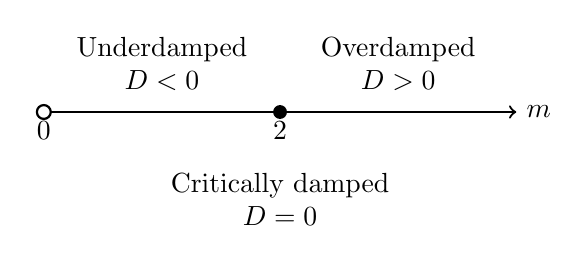
\begin{tikzpicture}[scale=1.0]
    % Parameter axis
    \draw[->,thick] (0,0) -- (6,0) node[right] {$m$};

    % Excluded endpoint and critical value
    \draw[fill=white,thick] (0,0) circle (2.5pt);
    \fill (3,0) circle (2.5pt);
    \node[below] at (0,0) {$0$};
    \node[below] at (3,0) {$2$};

    % Region labels
    \node[above,align=center] at (1.5,0.15)
        {Underdamped\\$D<0$};
    \node[above,align=center] at (4.5,0.15)
        {Overdamped\\$D>0$};

    % Critical-damping label
    \node[below,align=center] at (3,-0.65)
        {Critically damped\\$D=0$};
\end{tikzpicture}
\caption{This is the parameter space for the spring model in Example 2. Only $m>0$ is allowed. The mass $m=2$ acts as the critical value that separates underdamped from overdamped.}
\end{figure}

When two parameters can vary, we can represent all combinations in a \textbf{parameter plane}. Each point in the plane represents a specific setting for the spring setup. Our goal is to determine regions where the system is overdamped and underdamped.

\begin{example}[3]{
Consider the spring-mass equation
\[
mx''+\gamma x'+4x=0,
\qquad m>0,\quad \gamma>0.
\]
Sketch the regions in the $m\gamma$-plane where the system is
overdamped, critically damped, or underdamped.
}
The discriminant is
\[
D=\gamma^2-16m.
\]
Critical damping occurs when
\[
D=0
\quad\Rightarrow\quad
\gamma=4\sqrt{m},
\]
where we take the positive root because $\gamma>0$. To sketch the parameter space plot the curve
$$
    \gamma = f(m) = 4\sqrt{m} 
$$
on the $m\gamma$-plane. So $m$ on the horizontal axis and $\gamma$ on the vertical
axis. The curve $\gamma=4\sqrt{m}$ separates two regions:
\begin{itemize}
    \item Above the curve: $\gamma>4\sqrt{m}$, so $D>0$.
    The system is \textbf{overdamped}.
    \item On the curve: $D=0$.
    The system is \textbf{critically damped}.
    \item Below the curve: $0<\gamma<4\sqrt{m}$, so $D<0$.
    The system is \textbf{underdamped}.
\end{itemize}

\begin{figure}[H]
\centering
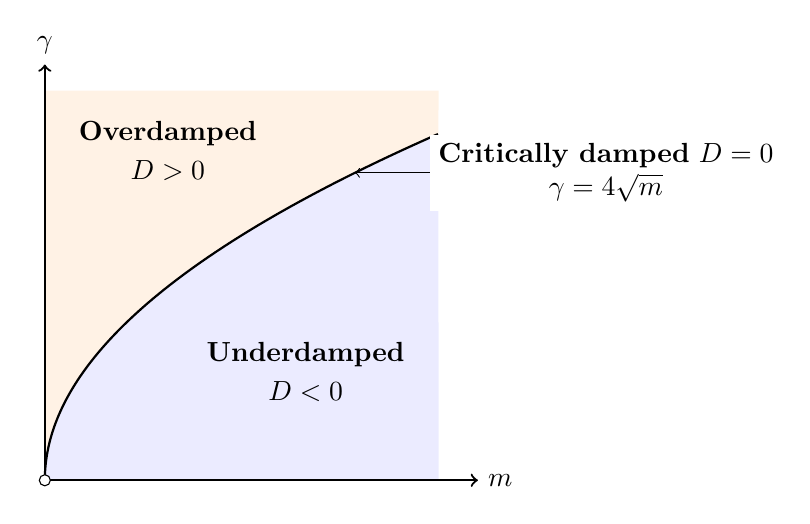
\begin{tikzpicture}[x=1.25cm,y=0.55cm]
    % Parameter regions
    \fill[blue!8]
        (0,0) -- plot[domain=0:4,samples=150]
        (\x,{4*sqrt(\x)}) -- (4,0) -- cycle;
    \fill[orange!10]
        (0,0) -- plot[domain=0:4,samples=150]
        (\x,{4*sqrt(\x)}) -- (4,9) -- (0,9) -- cycle;

    % Axes
    \draw[->,thick] (0,0) -- (4.4,0) node[right] {$m$};
    \draw[->,thick] (0,0) -- (0,9.6) node[above] {$\gamma$};

    % Critical-damping boundary
    % Parameterization m=s^2, gamma=4s
    \draw[thick,domain=0:2,samples=150,variable=\s]
        plot ({\s*\s},{4*\s});

    % Region labels
    \node[align=center] at (1.25,7.6)
        {\textbf{Overdamped}\\[2pt] $D>0$};
    \node[align=center] at (2.65,2.5)
        {\textbf{Underdamped}\\[2pt] $D<0$};

    % Boundary label
    \node[align=center,fill=white,inner sep=3pt]
        (critical) at (5.7,{4*sqrt(3.15)})
        {\textbf{Critically damped} $D=0$\\ $\gamma=4\sqrt{m}$};
    \draw[->] (critical.west) -- (3.15,{4*sqrt(3.15)});

    % Origin excluded
    \draw[fill=white] (0,0) circle (2pt);
\end{tikzpicture}

\end{figure}
\end{example}

%-------------------------------------------------------------

\section{Sketching Undamped Springs}
In this section, we will go over how to sketch solutions to $mx''+kx=0$.

\subsection{Phase--Amplitude Form}
In the undamped case $\gamma=0$, the model is
\[
m x'' + kx = 0.
\]
The characteristic roots are $\lambda=\pm i\omega$, where $\omega=\sqrt{\frac{k}{m}}$. The general solution is
\[
x(t)=c_1\cos(\omega t)+c_2\sin(\omega t).
\]
We call $\omega$ the \textbf{frequency} of the wave. The function is difficult to plot in its current form. It is easier to sketch the function when it is rewritten in \textit{phase-amplitude form}. 

\begin{theorem}
The function $x(t)=c_1\cos(\omega t)+c_2\sin(\omega t)$ can be written as
$$
x(t) = A \cos(\omega t-\varphi),
$$
where 
$$
A = \sqrt{c_1^2+c_2^2}, \quad \varphi = \arctan\frac{c_2}{c_1}.
$$
$A$ is called the \textbf{amplitude}. $\varphi$ is called the \textbf{phase angle} (with the appropriate quadrant adjustment).
\end{theorem}




\subsection{How to Sketch the Wave}
After writing the solution in phase-amplitude, factor out $\omega$ in the cosine term:
$$
x(t)=\underbrace{c_1\cos(\omega t)+c_2\sin(\omega t) }_{\text{solution}}=  \underbrace{A \cos(\omega t-\varphi)}_{\text{P.A. form}} = A \cos\underbrace{\left[\omega(t-\frac{\varphi}{\omega})\right]}_{\text{factor out }\omega}. 
$$
Factoring out $\omega$ reveals the \textbf{phase shift} $\tau=\frac\varphi\omega$. Think of $f(t)= A\cos(\omega t)$ as the base function, or the unshifted wave. The function $f(t)$ is simple to sketch by hand. Notice that $x(t) = f(t-\tau)$.  
\begin{enumerate}
    \item Calculate the value of $A$, $\varphi$, $\tau$, and the period $T=2\pi/\omega$.
    \item Lightly sketch the base function  $f(t)=A \cos\omega t$.
    \item Draw $A\cos(\omega(t-\tau))$ by shifting $f(t)$ $\tau$ units to the right.
    \item Make sure the sketch satisfies the ICs.
    \item Indicate the phase shift $\tau$ as the lag between the waves.
    \item Indicate the period $T$ as the distance between peaks.
\end{enumerate}



\begin{example}[4]{

Sketch the function 
$$
    x(t) = \cos 2t + \sqrt{3}\sin 2t,
$$
which is the solution to $x''+4x=0$ with ICs $x(0)=1$ and $x'(0)=2\sqrt{3}$.
}

First, we identify the values. In this solution, we have $\omega=2$, $c_1=1$, and $c_2=\sqrt{3}$. We will use these parameters to calculate the values:
$$
A = \sqrt{c^2_1+c^2_2}= 2,\quad \varphi = \arctan\frac{c_2}{c_1} = \frac{\pi}{3}, \quad T = \frac{2\pi}{\omega}=\pi,\quad \tau  =\frac{\varphi}{\omega}=\frac{\pi}{6}. 
$$
The function in phase-amplitude is 
$$x(t)=2\cos (2t-\frac{\pi}{3})=2\cos(2(t-\frac{\pi}{6})).$$
Next, lightly sketch the unshifted $2\cos(2t)$ on the $tx$-plane. Then sketch $2\cos(2(t-\frac{\pi}{6}))$ by shifting the wave $\frac{\pi}{6}$ units to the right.

\begin{figure}[H]
\centering
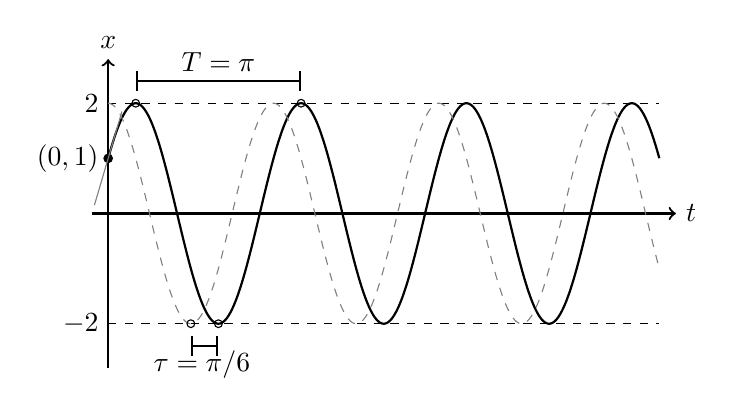
\begin{tikzpicture}[scale=0.7]
    \def\A{2}
    \def\T{3}        % 180 deg / 60 = 3
    \def\Tau{0.5}    % 30 deg / 60 = 0.5
    \def\uMax{10}    % shows 12*60 = 720 degrees
    \def\yMax{2.8}
    \def\yMin{-2.8}

    % Axes
    \draw[->,thick] (-0.3,0) -- (\uMax+0.3,0) node[right] {$t$};
    \draw[->,thick] (0,\yMin) -- (0,\yMax) node[above] {$x$};

    % Amplitude lines
    \draw[dashed] (0,\A) -- (\uMax,\A);
    \draw[dashed] (0,-\A) -- (\uMax,-\A);
    \node[left] at (0,\A) {$2$};
    \node[left] at (0,-\A) {$-2$};

    % Main curve: x(u) = 2 cos(120u - 60 deg)
    \draw[thick,domain=0:\uMax,samples=600]
        plot (\x,{\A*cos(120*\x - 60)});

    % Reference curve: 2 cos(120u)
    \draw[gray,dashed,domain=0:\uMax,samples=600]
        plot (\x,{\A*cos(120*\x)});

    % Initial point: t=0 -> u=0, x=1
    \fill (0,1) circle (2.5pt);
    \node[left] at (0,1) {$(0,1)$};

    % Tangent arrow (positive slope)
    \draw[thin,gray] (0,1) -- ++(0.25,0.85);
    \draw[thin,gray] (0,1) -- ++(-0.25,-0.85);

    % Phase shift line at tau = 0.5 (i.e., 30 deg)
    % \draw[dashed] (\tau,0) -- (\tau,\A);
    % \node[below] at (\tau,0) {$\tau=30^\circ$};

    \draw (\T/2,-\A) circle (2pt);
    \draw (\T/2+\Tau,-\A) circle (2pt);
    \draw[|-|,thick] (\T/2,-\A-0.4) -- (\T/2+\Tau,-\A-0.4);
    \node at (1.7,-\A-0.75) {$\tau=\pi/6$};
    
    % Mark peak to peak
    \draw (\Tau,\A) circle (2.0pt);
    \draw (\Tau+\T,\A) circle (2.0pt);
    \draw[|-|,thick] (\Tau,\A+0.4) -- (\Tau+\T,\A+0.4);
    \node at (2,\A+0.75) {$T=\pi$};

\end{tikzpicture}
\caption{This shows the plot of $x(t)=\cos 2t + \sqrt{3}\sin 2t$.}
\end{figure}
\end{example}


%-------------------------------------------------------------
\subsection{Warning About the Phase Angle}

You must be careful when using the formula
\[
\varphi = \tan^{-1}\!\left(\frac{c_2}{c_1}\right)
\]
because it does \emph{not} automatically give the correct angle. You must check the quadrant. Think of $(c_1, c_2)$ as a point in the $c_1c_2$-plane. The angle $\varphi$ is the angle made with the positive $c_1$-axis. Consider the following cases:
\begin{enumerate}
    \item If $c_1=4$ and $c_2=3$, then the formula gives
    \[
    \varphi_1 = \tan^{-1}\!\left(\frac{3}{4}\right) \approx 0.6435.
    \]
    This is in the first quadrant, so the calculator answer is correct.

    \item If $c_1=-4$ and $c_2=3$, then thoughtlessly entering the numbers into the calculator gives 
    \[
    \tan^{-1}\!\left(\frac{3}{-4}\right)
     \approx -0.6435,
    \]
    which is \textbf{very wrong}!. Since the point is in the 2nd quadrant, you must subtract the \textit{reference angle} from $\pi$. The correct angle is
    \[
    \varphi_2 = \pi - \underbrace{\tan^{-1}\!\left|\frac{3}{-4}\right|}_{\text{reference angle}}
    \approx 2.498.
    \]

    \item If $c_1=3$ and $c_2=-4$, the point lies in the fourth quadrant. In this case, you use the negative reference angle:
    \[
    \varphi_3 = -\tan^{-1}\!\left|\frac{-4}{3}\right|\approx -0.9273.
    \]
\end{enumerate}

\begin{figure}[H]
\begin{center}
    \centering
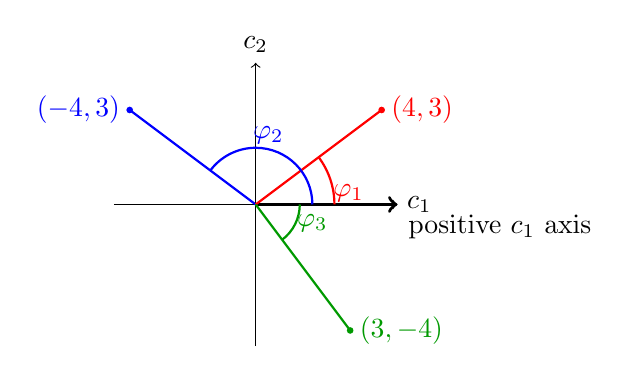
\begin{tikzpicture}[scale=0.4]
    % axes
    \draw[->] (-4.5,0) -- (4.5,0) node[right] {$c_1$};
    \draw[very thick,->] (0,0) -- (4.5,0) node[below right] {positive $c_1$ axis};
    \draw[->] (0,-4.5) -- (0,4.5) node[above] {$c_2$};
    % vectors
    \draw[thick,blue] (0,0) -- (-4,3);
    \fill[blue] (-4,3) circle (3pt);
    \node[blue,left] at (-4,3) {$(-4,3)$};
        % Angle arc Q1
    \draw[red,thick]
        (2.5,0) arc[start angle=0,end angle=36.87,radius=2.5];
    \node[red] at (2.95,0.35) {$\varphi_1$};

    \draw[thick,red] (0,0) -- (4,3);
    \fill[red] (4,3) circle (3pt);
    \node[red,right] at (4,3) {$(4,3)$};
    % Angle arc Q2
    \draw[blue,thick]
        (1.8,0) arc[start angle=0,end angle=143.13,radius=1.8];
    \node[blue] at (0.4,2.2) {$\varphi_2$};

    \draw[thick,green!60!black] (0,0) -- (3,-4);
    \fill[green!60!black] (3,-4) circle (3pt);
    \node[green!60!black,right] at (3,-4) {$(3,-4)$};
       \draw[green!60!black,thick]
        (1.4,0) arc[start angle=0,end angle=-53.13,radius=1.4];
    \node[green!60!black] at (1.8,-0.6) {$\varphi_3$};
\end{tikzpicture}
\end{center}
    \caption{If you draw the point $(c_1,c_2)$ on a plane, then $\varphi$ is the polar angle from the positive $c_1$ axis (counter clockwise is positive).}
\end{figure}

%-------------------------------------------------------------
\section{Sketching Underdamped Springs}
The goal of this section is to show how to sketch underdamped oscillators by hand. 

\subsection{Underdamped Solution}
In the underdamped case ($\gamma>0$ and $D<0$), the eigenvalues are
\[
\lambda=\alpha\pm i\omega
\quad\text{with}\quad \alpha<0,\ \omega>0.
\]
So the solution has contains a sum of waves which can be rewritten in phase-amplitude form 
\[
x(t)=e^{\alpha t}\bigl(\underbrace{c_1\cos(\omega t)+c_2\sin(\omega t)}_{\text{rewrite in P.A. form}}\bigr) =A e^{\alpha t}\cos(\omega t-\varphi).
\]
There are two differences from the undamped case: the wave is technically not periodic, the wave oscillates between two exponential functions. The oscillation still has a repeat time controlled by $\omega$:
\[
T=\frac{2\pi}{\omega}.
\]
We sometimes call this a \textbf{quasi-period} because the wave repeats in time, but the amplitude is shrinking, so the graph is not truly periodic. The underdamped wave bounces back and forth between the two \textbf{envelopes}:
$$
E_+(t) = Ae^{\alpha t},\quad E_-(t)=-Ae^{\alpha t}.
$$
These two functions represent the upper and lower bounds of the decaying wave.

\subsection{General Steps}
Here are the general steps:
\begin{enumerate}
    \item Write the wave in phase-amplitude form, if not given
    \item Draw the envelopes (the exponentials $\pm Ae^{\alpha t}$)
    \item Mark the initial point $(0,x_0)$ and indicate the slope $x'(0)=v_0$ 
    \item Draw a wave oscillating between the envelopes
    \item Indicate the distance between peaks with the quasi-period $T$
\end{enumerate}


\begin{example}[5]
{

Sketch the function 
$$
x(t) = e^{-t}(2\sin 3t -2 \cos 3t)
$$
with the given initial conditions $x(0)=-2$, $x'(0)=8$. 
}
Start by identifying the parameters 
$$
    c_1=-2,\quad c_2=2,\quad \omega=3.
$$
Next, we compute the three values for the phase-amplitude form:
$$
A=\sqrt{c^2_1+c^2_2} = \sqrt{8},\quad \varphi =\pi - \arctan\frac{|c_2|}{|c_1|}=\frac{3\pi}{4},\quad T=\frac{2\pi}{\omega}=\frac{2\pi}{3}.
$$
Note that the point $(c_1,c_2)=(-2,2)$ is in the 2nd quadrant, so we subtract the arctan angle from $\pi=180\degree$. Begin sketching the function by plotting the envelopes $ \pm\sqrt{8}e^{-t}$. Then label the initial position $(0,-2)$ with the slope $x'(0)=8$. Then draw the decaying wave bouncing between the envelopes. Finally, label the quasi-period $T$ as the horizontal distance between the peaks of the wave. 

\begin{figure}[H]
\centering
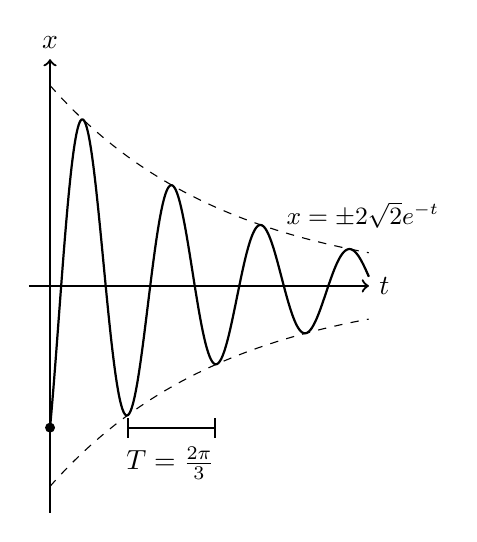
\begin{tikzpicture}[scale=0.9]

    % Parameters
    \def\A{2.828}    % 2sqrt(2)
    \def\a{-0.4}       % alpha
    \def\xMax{4.5}

    % Axes
    \draw[->,thick] (-0.3,0) -- (\xMax,0) node[right] {$t$};
    \draw[->,thick] (0,-3.2) -- (0,3.2) node[above] {$x$};

    % Envelopes
    \draw[dashed,domain=0:\xMax,samples=200]
        plot (\x,{\A*exp(\a*\x)});
    \draw[dashed,domain=0:\xMax,samples=200]
        plot (\x,{-\A*exp(\a*\x)});
    \node[right] at (3.2,1.0) {\small $x=\pm 2\sqrt{2}e^{-t}$};

    % Actual function
    \draw[thick,domain=0:\xMax,samples=400]
        plot (\x,{2.828*exp(\a*\x)*(cos(deg(5*\x-2.356)))});

    % Initial point
    \fill (0,-2) circle (2pt);
    % \node[left] at (0,-2) {$(-2)$};

    % Slope arrow at t=0
    % \draw[->,thick] (0,-2) -- (0.4,-1.2);

    % Quasi-period bracket
    \draw[thick,|-|] (1.083,-2) -- (2.34,-2);
    \node at (1.7,-2.5) {$T=\frac{2\pi}{3}$};

\end{tikzpicture}
\caption{This is a complete sketch of an underdamped wave. It has the envelopes, the IC, and the quasi-period.}
\end{figure}
\end{example}


\end{document}
